% Chapter 2. The host is the trust boundary. Not the model.
\documentclass[tikz,border=6pt]{standalone}
% Shared look for every TikZ figure in the book.
% Colours match book/preamble.tex exactly. Change both or neither.

\usepackage{tikz}
\usepackage{xcolor}
\usepackage{amsmath}
\IfFileExists{libertinus.sty}{\usepackage[mono=false]{libertinus}}{}
\IfFileExists{inconsolata.sty}{\usepackage[varqu,varl,scaled=0.95]{inconsolata}}{}

\usetikzlibrary{
  arrows.meta, positioning, calc, fit, backgrounds, shapes.geometric,
  shapes.misc, decorations.pathreplacing, decorations.pathmorphing,
  patterns, chains, matrix, shadows.blur
}

\definecolor{ink}{HTML}{15181D}
\definecolor{muted}{HTML}{5B6472}
\definecolor{rule}{HTML}{C9CED6}
\definecolor{wash}{HTML}{F4F5F7}
\definecolor{accent}{HTML}{0F5C8C}
\definecolor{accentsoft}{HTML}{E7F0F6}
\definecolor{warm}{HTML}{B4531A}
\definecolor{warmsoft}{HTML}{FBF0E7}
\definecolor{good}{HTML}{2C6E49}
\definecolor{goodsoft}{HTML}{E9F2EC}
\definecolor{danger}{HTML}{9B2226}
\definecolor{dangersoft}{HTML}{FAECEC}

\tikzset{
  font=\sffamily\small,
  >={Stealth[length=5pt, width=4pt]},
  %
  box/.style={
    draw=rule, line width=0.8pt, fill=wash, rounded corners=2pt,
    inner sep=7pt, align=center, text=ink, minimum height=9mm,
  },
  boxa/.style={box, draw=accent, fill=accentsoft},
  boxg/.style={box, draw=good,   fill=goodsoft},
  boxw/.style={box, draw=warm,   fill=warmsoft},
  boxd/.style={box, draw=danger, fill=dangersoft},
  %
  lane/.style={draw=rule, line width=0.7pt, fill=white, rounded corners=2pt,
               inner sep=6pt, align=center, minimum width=26mm},
  %
  flow/.style={draw=accent, line width=1.0pt, ->},
  flowback/.style={flow, densely dashed},
  flowmuted/.style={draw=muted, line width=0.8pt, ->},
  lifeline/.style={draw=rule, line width=0.7pt, densely dotted},
  %
  lbl/.style={font=\sffamily\scriptsize, text=muted, inner sep=2pt},
  lblink/.style={font=\sffamily\scriptsize, text=ink, inner sep=2pt},
  tag/.style={font=\ttfamily\scriptsize, text=accent, inner sep=2pt,
              fill=white, inner xsep=3pt},
  note/.style={font=\sffamily\scriptsize\itshape, text=muted, align=left},
  %
  band/.style={draw=none, rounded corners=1pt},
  tick/.style={draw=muted, line width=0.6pt},
}

% A horizontal timeline bar segment: \barseg{x0}{x1}{y}{colour}{label}
\newcommand{\barseg}[5]{%
  \fill[#4, rounded corners=1pt] (#1,#3-0.16) rectangle (#2,#3+0.16);
  \node[lbl, text=white, font=\sffamily\scriptsize\bfseries]
       at ({(#1+#2)/2},#3) {#5};
}

\begin{document}
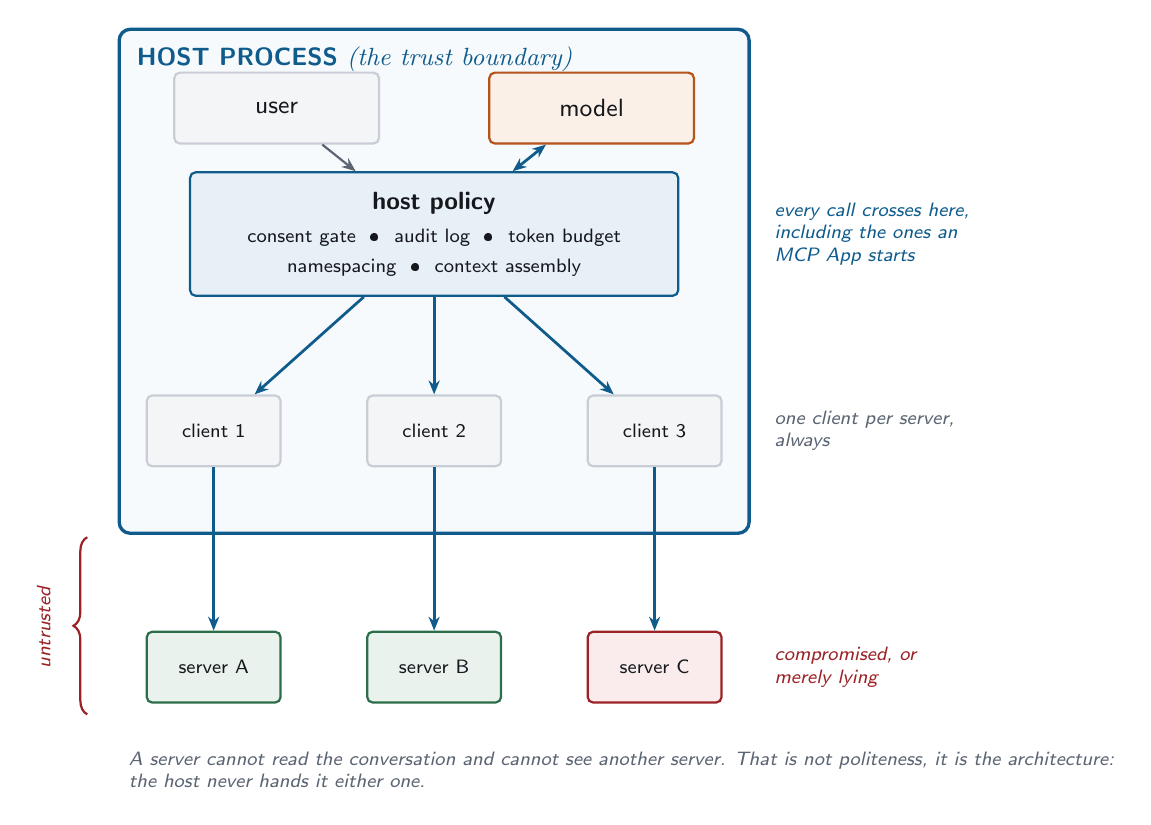
\begin{tikzpicture}[x=1cm, y=1cm]

  % --- the host process --------------------------------------------------
  \draw[draw=accent, line width=1.2pt, rounded corners=4pt, fill=accentsoft, fill opacity=0.35]
    (-0.6,-2.9) rectangle (7.4,3.5);
  \node[anchor=north west, font=\sffamily\bfseries\small, text=accent]
    at (-0.5,3.4) {HOST PROCESS \normalfont\itshape(the trust boundary)};

  \node[box, minimum width=26mm] (user) at (1.4,2.5) {user};
  \node[boxw, minimum width=26mm] (model) at (5.4,2.5) {model};

  \node[boxa, minimum width=62mm, align=center] (policy) at (3.4,0.9)
    {\textbf{host policy}\\[1pt]
     \scriptsize consent gate \ \textbullet\ \ audit log \ \textbullet\ \ token budget\\
     \scriptsize namespacing \ \textbullet\ \ context assembly};

  \node[box, minimum width=17mm, font=\sffamily\scriptsize] (cl1) at (0.6,-1.6) {client 1};
  \node[box, minimum width=17mm, font=\sffamily\scriptsize] (cl2) at (3.4,-1.6) {client 2};
  \node[box, minimum width=17mm, font=\sffamily\scriptsize] (cl3) at (6.2,-1.6) {client 3};

  \draw[flowmuted] (user) -- (policy);
  \draw[<->, draw=accent, line width=1pt] (model) -- (policy);
  \foreach \c in {cl1,cl2,cl3} { \draw[flow] (policy) -- (\c); }

  % --- the servers, outside the boundary ---------------------------------
  \node[boxg, minimum width=17mm, font=\sffamily\scriptsize] (s1) at (0.6,-4.6) {server A};
  \node[boxg, minimum width=17mm, font=\sffamily\scriptsize] (s2) at (3.4,-4.6) {server B};
  \node[boxd, minimum width=17mm, font=\sffamily\scriptsize] (s3) at (6.2,-4.6) {server C};

  \draw[flow] (cl1) -- (s1);
  \draw[flow] (cl2) -- (s2);
  \draw[flow] (cl3) -- (s3);

  \node[note, anchor=west, text=danger, align=left] at (7.6,-4.6)
    {compromised, or\\merely lying};

  % --- the invariants ----------------------------------------------------
  \node[note, anchor=west, align=left, text=muted] at (7.6,-1.6)
    {one client per server,\\always};

  \node[note, anchor=west, align=left, text=accent] at (7.6,0.9)
    {every call crosses here,\\including the ones an\\MCP App starts};

  \draw[decorate, decoration={brace, amplitude=5pt, raise=3pt}, danger, line width=0.8pt]
    (-0.9,-5.2) -- (-0.9,-2.95);
  \node[note, text=danger, rotate=90, anchor=south] at (-1.35,-4.1)
    {untrusted};

  \node[note, anchor=north west, align=left, text=muted] at (-0.6,-5.55)
    {A server cannot read the conversation and cannot see another server.
     That is not politeness, it is the architecture:\\the host never hands it
     either one.};

\end{tikzpicture}
\end{document}
